\section{Introduction}
\label{sec:introduction}

Retrieval-augmented generation (RAG) has become a standard paradigm for grounding large language models in external knowledge sources~\cite{lewis2020retrieval,gao2023retrieval}. A RAG system retrieves documents or passages for a user question and conditions a generator on the retrieved context. This interface makes RAG attractive for knowledge-intensive question answering, enterprise assistants, scientific search, and attributed generation, where users expect answers to be both useful and inspectable.

However, document relevance is not the same as answer support. A retrieved passage can be relevant to the question but fail to support a particular factual statement in the generated answer. A citation can support one fact in a sentence while leaving another fact unsupported. A generator can also combine retrieved content with unsupported parametric knowledge. These failures are common in long-form and attributed generation, where a single answer may contain many atomic factual claims with different evidence needs~\cite{gao2023enabling,wallat2025correctness}.

The key limitation is that many RAG systems are controlled at the level of queries, documents, passages, or whole responses, while faithfulness failures occur at the level of individual answer claims. Consider a question that asks for several attributes of an entity. A retriever may find evidence for some attributes but not others. The generator may nevertheless produce a complete-looking answer by filling the missing attribute from parametric knowledge or by copying a weakly related passage. A sentence-level citation checker may observe that the sentence has a citation, but this does not imply that every atomic claim in the sentence is entailed by the cited source.

We argue that reliable RAG requires an explicit \emph{claim-level evidence coverage} state: which answer units are already supported, which claims are unsupported, which claims lack citations, which citations point to the wrong evidence, and which answer units remain missing. This state should not only be used for post-hoc evaluation. It should control how the system spends additional retrieval, verification, and generation budget.

We propose \textsc{CoverRAG}, a coverage-guided claim verification controller for plug-and-play RAG. Given a draft answer from any RAG backbone, \textsc{CoverRAG} decomposes the answer into atomic claims, verifies each claim against evidence, and builds a coverage state over supported and unresolved answer units. Supported claims form an intermediate supported answer. Unsupported, uncited, or wrongly cited claims reveal possible coverage gaps. The controller then plans concrete missing answer-unit targets, retrieves or selects evidence only for those targets, and accepts a new claim only if it both fills a missing answer unit and is supported by evidence.

\begin{figure}[t]
    \centering
    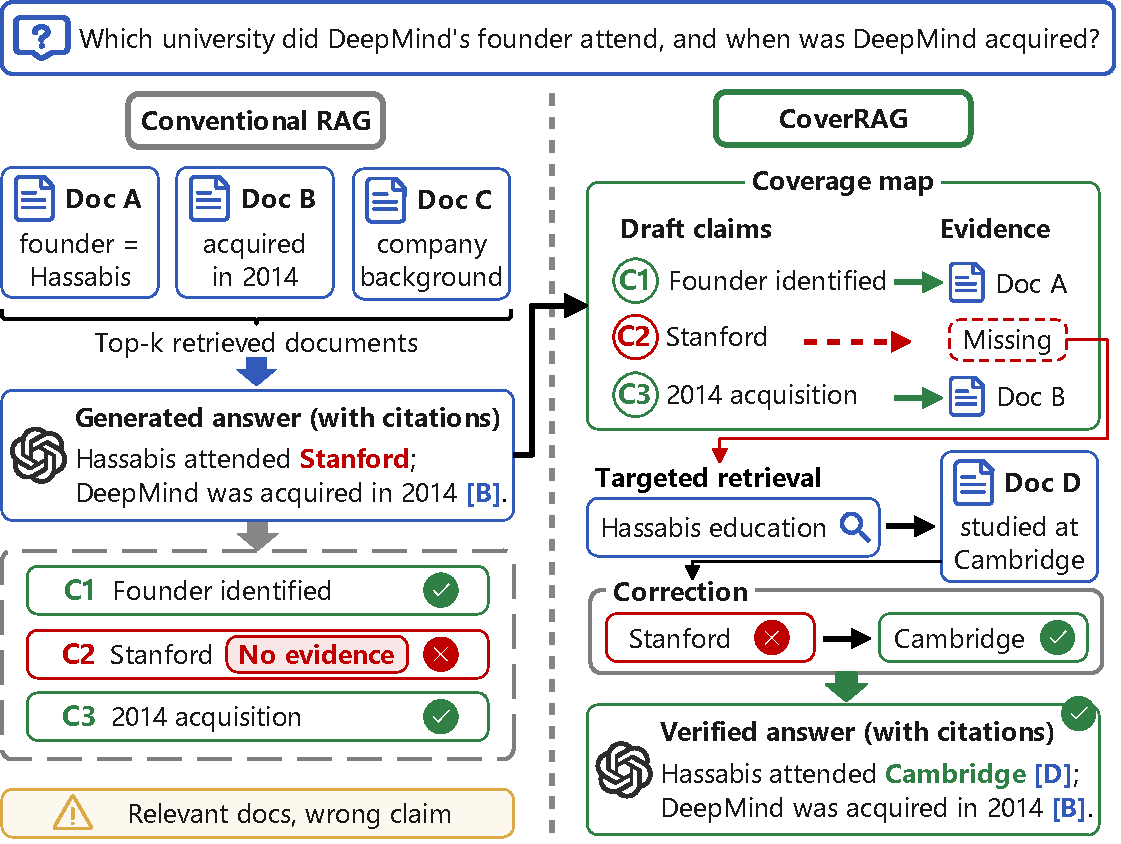
\includegraphics[width=\linewidth]{figs_wh/bg.pdf}
    \caption{Conventional RAG optimizes retrieved context for the original query. \textsc{CoverRAG} instead maintains a claim-level coverage state and uses unresolved answer units to guide retrieval, verification, and guarded answer update.}
    \label{fig:motivation}
\end{figure}

\autoref{fig:motivation} illustrates the distinction. Standard RAG produces an answer from an initial evidence pool. \textsc{CoverRAG} treats that answer as a hypothesis to be audited. The controller asks: which claims are supported, which answer units remain missing, and which new claims can be safely added without degrading citation faithfulness? Retrieval is then targeted by the original question, the missing answer unit, optional evidence clues, and the already supported answer state. This discourages redundant search for already covered content and focuses the evidence budget on unresolved answer units.

The design is plug-and-play. \textsc{CoverRAG} does not require modifying the internals of the base retriever or generator. It only assumes access to a draft answer and a candidate evidence pool. We instantiate it on three backbones: vanilla RAG, Self-RAG~\cite{asai2024self}, and BGE-rerank RAG. These backbones differ in how they generate the draft answer; \textsc{CoverRAG} adds the same answer-side coverage controller after generation.

Our evaluation uses ASQA, ELI5, and QAMPARI from the attributed long-form generation setting~\cite{gao2023enabling}. We report task correctness and task recall, sentence-level citation recall and precision, claim-level citation recall and precision, claim sentence recall, and claim support. This evaluation is necessary because a system can improve citation precision by deleting information, or improve support by adding facts that are supported but irrelevant. \textsc{CoverRAG} is designed to improve claim support and citation faithfulness while preserving useful answer content.

This paper makes the following contributions:

\begin{itemize}
    \item We formulate RAG answer refinement as \emph{claim-level evidence coverage}, explicitly tracking supported, unsupported, uncited, and wrongly cited atomic answer claims.
    \item We introduce \textsc{CoverRAG}, a coverage-guided iterative controller that plans missing answer-unit targets, retrieves or selects evidence for those targets, and accepts new content only when it is both coverage-improving and evidence-supported.
    \item We demonstrate plug-and-play effectiveness across vanilla RAG, Self-RAG, and BGE-rerank RAG on three attributed generation datasets, showing large gains in claim support and citation faithfulness while preserving or improving main task performance.
\end{itemize}

Overall, \textsc{CoverRAG} advances a simple view: trustworthy RAG should not only retrieve relevant documents, but should optimize the coverage relation between answer claims and supporting evidence.

